\documentclass[12pt,titlepage,french]{article}
\usepackage{babel}
\usepackage{graphicx}
\usepackage[margin=2.5cm]{geometry}
\usepackage{tabularx}
\usepackage[hidelinks]{hyperref}

\usepackage[utf8]{inputenc}
\usepackage[T1]{fontenc}
\pagestyle{plain}

\usepackage{booktabs,makecell,tabu}
\renewcommand\theadfont{\bfseries}

\linespread{1.5}

\begin{document}

\begin{titlepage}
\newcommand{\HRule}{\rule{\linewidth}{0.5mm}}
\center

  
\includegraphics[width=0.45\textwidth]{../ressources/img_logos/logo_polytech.png}\\[1cm]
   
  
\includegraphics[width=0.45\textwidth]{../ressources/img_logos/logo_taglabs.png}


\HRule \\[0.4cm]
{ \huge \bfseries Description du système \\[0.15cm] }
Classification colorimétrique de nuages de points 3D
\HRule \\[1.5cm]
Ronan Collier,
Mathieu Letrone,
Tri-Thien Truong
\\[1cm]
\today \\ [1cm]
Version 1.0 - Alpha
\end{titlepage}

\tableofcontents % table des matières
\newpage
\listoffigures  % table des figures
\newpage
\section{Contexte et problème}

Taglabs est une jeune entreprise créée il y a deux ans par Yan Koch. L’entreprise s’inscrit dans le domaine de la modélisation 3D d’ouvrages. Ils proposent la modélisation et l’exploitation de nuages de points. Toutefois, ils travaillent surtout en interne sur un logiciel « ScanSap », le but de ce logiciel est d’exploiter les nuages de points 3D avec efficacité et simplicité inégalées.

Voulant continuer leur développement dans ce domaine encore nouveau, l'entreprise cherche maintenant à améliorer leurs outils, afin de compléter l'exploitation des nuages de points. L'ensemble de ces fonctionnalités permettent à leurs clients de pouvoir analyser un environnement en numérique, à un instant précis (qui sera sous la forme d'un scan de nuages de points). Par exemple, une entreprise peut avoir le besoin d'avoir un scan d'une de leur usine, afin d'analyser le positionnement de leurs machines, les potentielles fuites au niveau des tuyaux, etc.

Dans cette optique, l'entreprise souhaite pouvoir intégrer plusieurs fonctionnalité à son système. D'une part, une solution permettant une segmentation basé sur la couleur au sein du ou des nuages de points manipulés. Cette segmentation a pour but de mettre en évidence, isolé les éléments du nuage de point répondant à une plage de couleur demandée. D'autre part, une solution mettant en place une fausse couleur sur un scan (nuage de points) en intensité. Le rôle de la fausse couleur est de mettre en lumière des caractéristiques issu des éléments scannés, et de facilité la compréhension général du nuage en y mettant des couleurs.

l'ensemble des fonctionnalités demandées par le client est une demande de recherche algorithmique sur l'implémentation des solutions. 
\newpage
\section{Solution mise en place : vue globale}

Dans cette partie nous allons présenter l'ensemble des choix que nous avons fait afin de répondre au mieux aux besoins demandés par le client. Et la description de la solution conçue  pour satisfaire lesdit besoins.

\subsection{Choix principaux}

%/!\ 
% Donner vos choix principaux (service, techno, etc.), en expliquant pourquoi vous les avez fait. 
%/!\
Afin de répondre aux besoins, qui sont de pouvoir :
\begin{itemize}
    \item Lire un fichier de données contenant un nuage de point.
    \item Isoler un élément dans le nuage de points, selon sa plage de couleur.
    \item Réaliser de la fausse couleur sur un nuage de points en intensité de gris.
    \item Exporter le nuage de points.
\end{itemize}
Le service proposé doit permettre aux utilisateurs de réaliser ces tâches. Nous avons d'abord défini en tant qu'utilisateurs de la solution, ceux qui utiliseront "ScanSap" qu'il s'agisse de client ou de membre de l'entreprise TagLabs. Ainsi, nous visons des utilisateurs voulant manipuler des nuages de point en 3D, ces personnes sont équipés de matériels puissants pour cela.
% Dire qu'on se tourne donc ni vers service web ou mobile (puissance de calcul nécessaire) ?
% implicite car ScanSap application bureau
N'existant pas outil permettant l'ajout direct de fonctionnalités extérieures au sein du logiciel "ScanSap", nous avons décidé avec l'entreprise de réaliser un plugin sur autre logiciel de manipulation de nuages de points. Le logiciel en question est CloudCompare, il permet la manipulation et le traitement des nuages, de plus, sa licence open source autorise l'ajout de fonctionnalités tant que nous les livrons aussi en open source.

Cette décision fut prise pour répondre non seulement à l'ensemble des besoins, mais aussi car CloudCompare prend déjà en charge deux besoins, la lecture et l'exportation des scans. En faisant ce choix, nous pouvons nous consacrer à la recherche et réalisation des autres besoins de la segmentation et de la fausse couleur demandés par l'entreprise.
%, tout en proposant une solution moins complète mais fonctionnelle à l'ensemble des utilisateurs de CloudCompare. ?

% <Rajouter quelque chose ?>

%>>>>>>>>>>>>>>>>>>>>>>>>Version 1.0<<<<<<<<<<<<<<<<<<<<<<<<
% Ce qui est dit est sûrement pas ce qui est demandé

%Après une phase de recherche et discussion entre les différents partis du projet. Nous nous sommes orientés non plus sur une phase seulement algorithmique mais sur l'implémentaion de nos solutions via un plugin sur un logiciel de manipulation de nuages de points nommés CloudCompare. Ce choix a été fait pour se concentrer davantage sur les algorithmes des solutions que l'implémentation des méthodes de lecture/export de nuages de points.
%/!\
% Partir du / des besoins pour expliquer ce qu'on fait (plugin répond à quel besoin)
% diagrammes de séquence sur les users case/stories

%Le fait de travailler sur cloudCompare à orienté beaucoup de nos choix sur l'environnement de travail et les technologies utilisées. En effet, au vu des nombreuses dépendances, des incations données sur la page git du logiciel, nous avons utilisé Cmake. CMake est système qui permet la vérification des pré-requis nécessaires avant la construction, de déterminer les dépendances afin de planifier la construction adapté à la plateforme.
% %j'avoue que je sais pas si c'est vraiment nécessaire de le dire

%Pour ce qu'il en est du choix du langage, compte tenu que nous développons un plugin sur CloudCompare, il a fallut opter pour le langage qui parviendra au mieux à l'implémentation dudit plugin. Le choix se faisait entre le C++ et le Python, (le tableau compartif est disponible dans le rapport de l'itération une), la décision fut le C++, pour cause, l'ensemble du logiciel est en C++, ce qui permettra de simplifier l'interfaçage et la création du plugin. 

% %j'ai l'impression de tourner en rond

%Le langage étant rapide et compatible avec de nombreuses bibliothèques. Nous avons décidé de réaliser entièrement le projet en C++, et ainsi éviter de gérer des dépendances uniquement pour la création d'algorithmes en Python.
%Pourquoi c++, et CloudCompare 
%<<<<<<<<<<<<<<<<<<<<<<<<<<<<<<<<<<<<<<<<<<<<<<>>>>>>>>>>>>>>>>>>>>>>>>>>>>>>>>>>>>>>>>>>>>>>>>>
\newpage
\subsection{Description de la solution}
%/!\ 
% Décrivez notamment quel est le service offert pour répondre à la problématique (How?), et ce qu’est votre solution concrètement (What?).
%/!\
Comme dit précédemment la solution proposée pour répondre à la problématique s'articule autour d'un service de type plugin utilisateur. Le plugin est intégré dans les composants tiers de CloudCompare, il comprends (comprendra) les fonctionnalités de segmentation suivant la plage colorimétrique et la génération de fausse couleur sur un scan en intensité. Les utilisateurs pourront y accéder en les sélectionnant dans le menu défilant qui liste les différents plugins présents. Les diagrammes de séquence qui suivent, détaillent le fonctionnement et l'expérience utilisateur.



\begin{figure}[!hbtp]
\center
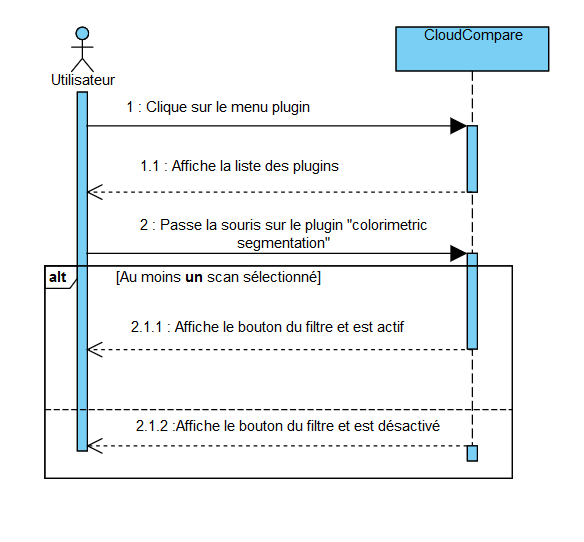
\includegraphics[width=0.65\textwidth]{sequDiagPlugin.PNG}
    \caption{\label{} Diagramme de séquence sur l'accès au plugin}
    
  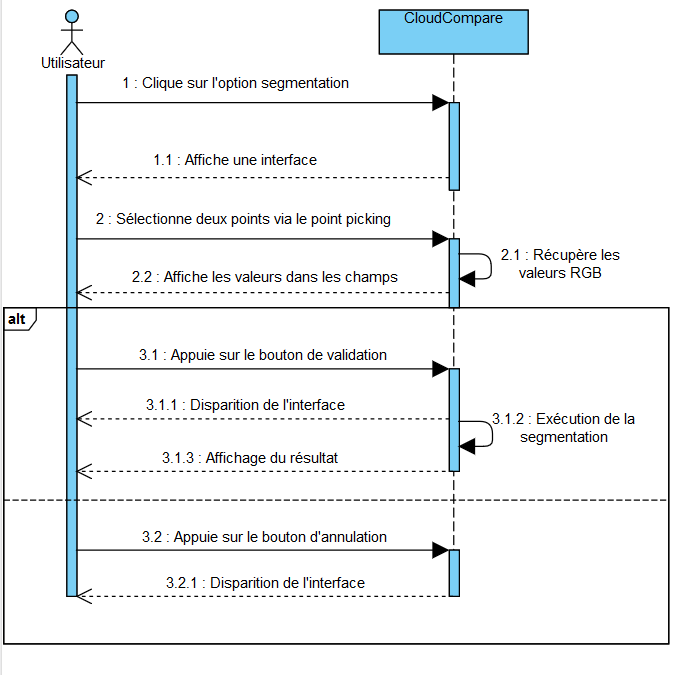
\includegraphics[width=0.65\textwidth]{sequDiagrSegmentation.PNG}
  \caption{\label{} Diagramme de séquence sur l'utilisation de la segmentation}
\end{figure}

\section{Description technologique de la solution}
Notre solution étant un plugin pour CloudCompare, la principale difficultée technique est la compréhension de la structure de ce logiciel et de son API.
En effet, CloudCompare possède une structuration complexe pour quiconque n'est pas habitué à travailler sur des projets C++ d'une telle envergure.
De plus, la documentation possède de nombreuses lacunes, ne présentant pas toutes les classes et n'étant pas à jour. La seule documentation disponible est en ligne et nous n'avons.
Il est donc conseillé de regarder le fonctionnement de l'API en naviguant dans les sources du projet.
Le code source du projet se trouve aux côtés de celui des autres plugins, dans le dossier "plugin" situé à la racine du dossier des sources de CloudCompare.
Chaque sous-dossier de ce dossier représente un plugin.\newline
Le fichier le plus important pour la compilation du projet est le "CMakeLists.txt". En effet, il contient le nom de la classe principale du projet ainsi que tout les fichiers à inclure lors de la compilation.
Si la structure du projet est correct, et les fichiers correctements configurés, une option sélectionnable apparait dans CMake. 
Il est alors possible de construire le projet pour qu'il soit éditable à l'aide de QtCreator tout autre IDE (tel que Visual Stuio, en sélectionnant l'option appropriée).
Notre classe principale est ainsi nommée "ColorimetricSegmenter". Etant donné que notre projet est en C++, la classe est d'abord représentée sous la forme d'un fichier de type "header", contenant simplement les signatures des méthodes. 
Afin de pouvoir intéragir avec l'environnement de cloudCompare, il a fallu faire hériter notre classe de la classe "ccStdPluginInterface".\newline
L'interface graphique de cloudCompare se base sur la bibliothèque Qt. Cette bibliothèque offre plusieurs moyens afin de créer de nouveaux panneaux d'interface, de les intégrer à l'environnement existant, et de les lier à des actions.
QtCreator permet de concevoir graphiquement un panneau au travers une interface intuitive en drag\&drop. Le panneau nouvellement créé peut être enregistré au format XML avec l'extension ".ui".
Lors de la génération du projet, des fichiers ".h" et ".cpp" sont automatiquement créés par cloudCompare afin de pouvoir ouvrir la fenètre et manipuler ses champs.\newline
Les actions utilisateurs sont également géré gràce à Qt au travers de la mécanique des signaux.

\newpage
\section{Conclusion et perspectives}
% 2-3 pages
% Faire le bilan global du projet (sur les itérations décrites, pour le rapport alpha)
% Donnez les perspectives pour la suite (pour les prochaines itérations, sur le rapport alpha)

Nous avons jusqu'à maintenant réalisé la moitié du projet, au niveau du temps. En effet, nous avons maintenant passé trois itérations sur l'élaboration de notre solution. \newline

Pour conclure sur ces itérations, de façon générale, nous avons pu suivre en grande partie ce que nous avions prévu sur le cahier des charges. La majorité des Users Stories ont été développés et validés par le client. Toutefois, le projet est loin d'être terminé, et il nous reste encore beaucoup d'améliorations/implémentation de fonctionnalités à faire.

La première itération nous a permis de nous conforter sur le développement futur de notre solution, et les deux autres nous ont permit de poser les bases, et de commencer à donner une solution viable.

Durant la première itération, nous avons de nombreuses questions sur le développement de notre projet. Nous avions notamment le choix du langage, la façon de développer nos algorithmes, l'implémentation, etc. C'était une itération où nous n'avions pas produit de contenu direct pour le client, mais nous avions pu partager nos recherches et de nos choix. Nous avions donc décidé de développer notre solution en C++, avec un plugin CloudCompare. 

La recherche d'algorithmes de segmentation nous a permis de gagner du temps sur l'implémentation, afin d'éviter de changer entre phases de recherche, et phases de d'implémentation, sur une même itération. Ainsi, cela nous permettait de mieux se concentrer sur la phase d'implémentation. 

Toutefois, nous avons quand même pris du retard notamment sur la deuxième et troisième itération. Lors de la deuxième itération, nous pensions que nous pourrions avoir une meilleure base de notre plugin sur CloudCompare, afin de pousser l'implémentation des algorithmes de segmentation. Malheureusement, nous avions rencontré des difficultés par rapport à la création d'un nouveau plugin. Ce temps perdu a donc impacté le développement de la troisième itération, qui consistait à l'amélioration de ce que nous avions développé, et l'implémentation de nouveaux algorithmes.

Lors de la troisième itération, nous avions préféré se concentrer sur l'amélioration de notre code par rapport à l'implémentation de nouvelles fonctionnalités, car il nous semblait important d'avoir une structure stable et facile à maintenir, pour la suite du projet. Grâce à cela, nous avons maintenant un plugin indépendant aux autres, qui est totalement fonctionnel, et qui peut facilement ajouter des nouveaux algorithmes de segmentation. 

De plus, nous avons quand même pris en compte le feedback du client, afin d'améliorer notre solution, par rapport à son utilisation. Ici, c'était principalement lié à l'interface des algorithmes de segmentation. Nous avons apporté des modifications notamment sur le point picking, très important pour faciliter l'utilisation de notre plugin (au lieu de rentrer manuellement les valeurs à filtrer), ou encore des changements sur la plage de couleur à prendre, etc. \newline

Maintenant, nous devons réfléchir aux perspectives d'évolution du projet. Il nous reste maintenant trois itérations à planifier, pour finaliser notre solution. \newline

Nous avions encore des tâches non terminées, que nous devons finir. Ces tâches sont le développement d'un nouvel algorithme pour réaliser le filtrage des points, et d'améliorer le filtrage via l'espace de couleur CieLAB, afin de voir si cette solution est viable. Ces deux tâches sont donc à prioriser dans le développement, qui seront donc dans notre quatrième itération.

De plus, nous devons prendre en compte les retours du client. Ici, le principal retour a été par rapport à la marge d'erreur, que l'utilisateur se fixe afin de créer ses plages de couleurs à filtrer. Ce système de marge d'erreur est à revoir. Il est en effet peu parlant pour un utilisateur et peu pertinent suivant les cas d'utilisations. Si les valeurs sont faibles, "la marge" en sera impactée et réduite. Au lieu, d'avoir cette marge, il serait mieux de choisir/sélectionner deux points dans le nuage, l'un serait la borne "basse" et l'autre la borne "haute". On choisirait ainsi, l'espace de couleur qu'on choisit de segmenter.

Ensuite, la possibilité de réaliser un premier process sur le nuage avant la segmentation, permettrait de discrétiser l'histogramme des couleurs, pour obtenir un effet cartoonesque. De ce fait, le problème des contrastes et différentes luminosités seraient déjà grandement palliés en plus de donner une meilleure idée des éléments gardés après la segmentation.

Ces retours sont très intéressants, et nous pensons que ces tâches sont aussi importantes à prendre en compte pour l'amélioration de notre solution. \newline

D'autres tâches sont encore en suspend, que nous avions planifié dans le cahier des charges. La principale tâche est la fausse couleur, que nous avions planifié pour la quatrième itération. Nous voulons le faire assez tôt afin d'avoir le feedback du client, et de l'améliorer sur les futures itérations.

L'autre tâche est de potentiellement traiter le problème du mouchetage, que l'on peut rencontrer lors de fusion de nuage de points. Comme cette tâche n'était pas la priorité du client, nous ne savons encore pas si nous allons faire des recherches sur ce cas. Toutefois, elle reste dans notre backlog et pourra être traité dans nos futures itérations.

\section{Annexes}

\subsection{Déroulement du projet}
% retour rétrospectif sur la manière dont le projet s'est déroulé, points forts et difficultés, changement de méthode en cours de route, etc. pour :
% - le projet global, la phase de réalisation (5 itérations), les itérations.
% Pour chaque itération, produire un gantt prévisu sous forme d'un simple tableau (tâche prévue, temps, responsable), et un gantt réalisé + analyse de différence

\subsubsection{Vision globale du projet}

Il est important de faire un retour sur le déroulement du projet, afin de savoir ce que nous avons bien réalisé, les difficultés que nous avons rencontrés, nos méthodes de travail, etc. En effet, cela nous permettra d'améliorer nos démarches pour mener à bien ce projet. \newline

D'un point de vu global sur le projet, sur ces trois premières itérations, nous avons rencontré certaines difficultés, mais aussi appris beaucoup par rapport au fonctionnement d'un projet agile.

Tout d'abord, il a été difficile d'estimer notre charge de travail. Comme c'était notre premier vrai projet en lien avec une autre entreprise, et d'une aussi grande envergure (durée d'un an), il nous fallait en quelque sorte expérimenter notre capacité de travail et d'évaluer les tâches à réaliser.

Certaines tâches furent plus difficiles à réaliser, par rapport à nos prévisions. Par exemple, nous pouvons citer l'implémentation d'un nouvel algorithme de segmentation, plus complexe, ou encore l'implémentation d'un point picking. Le temps prévu à consacrer sur ces types de tâches n'était pas assez important, car nous avions mal pris en compte les autres tâches en parallèle, hors projet. Ces autres tâches était notamment d'autres projets sur de courtes durées, devoir surveillées, oraux, etc. \newline

Nous nous sommes aussi rendu compte que les itérations se déroulent très vite. Pour chaque itération, nous étions surpris par le fait qu'un mois s'était passé. Grâce aux réunions planifiées avec le client et le tuteur académique, nous pouvions quand même garder une bonne dynamique pour respecter les deadlines. \newline

De plus, la mise en situation d'un projet agile nous a fait prendre conscience de l'importance de garder le client au courant, afin d'avancer correctement par rapport aux besoin de celui-ci. Mais pour cela, il faut rédiger de nombreux rapports. Ce sont des tâches qu'il ne faut pas sous-estimer, puisque cela demande beaucoup de temps. Même si les réunions aident à transmettre l'avancement du projet et des tâches réalisées, il faut aussi écrire formellement dans un rapport l'avancement pour garder une trace de ce qui a été fait.

La rédaction des rapports d'itération, et des rapports hebdomadaires, sont difficiles à maintenir. En effet, nous avions eu parfois des difficultés à suivre le rythme des rapports hebdomadaires. Malgré tout, cela reste nécessaire notamment pour avoir un historique de l'avancement des tâches, et des heures passées sur chacune d'entre elles.

\subsubsection{Comparaison de la planification des itérations}

\subsection{Rapport de recette}

Cette section sera présente pour le rapport final de la description du système (version beta).

\end{document}
